\chapter{Overview of Netconf}

Along this chapter we will describe the operation of \gls{NETCONF}, indicating the tole played by the solutions mentioned above: \gls{YANG}, \gls{XML}, and \gls{RPC}.  

\section{Network Configuration Protocol - NETCONF}

\gls{NETCONF} is an Internet Engineering Task Force (IETF) network management protocol that provides a secure mechanism for installing, manipulating and deleting the configuration data on a network device, such as a firewall, router or switch.
NETCONF was developed by the NETCONF working group and published in December 2006 as RFC \cite{rfc4741}. The protocol was then revised in June 2011 and published as RFC 6241 \cite{rfc6241}, which is the most current version. The IETF also published several other RFCs related to NETCONF. For example, RFC 5277 \cite{rfc5277} defines a mechanism for supporting an asynchronous message notification service for NETCONF.
The NETCONF protocol was designed to make up for the shortcomings of the Simple Network Management Protocol and the command-line interface scripting used to configure network devices.

NETCONF uses the Remote Procedure Call (RPC) protocol to carry out communications between clients and servers. RPC is a client/server protocol that lets a program request a service from another one without understanding the details of the underlying network. RPC messages are encoded in Extensible Markup Language (XML) and transmitted via secure connection-oriented sessions.
A NETCONF client, which is often part of a network manager, can be a script or application. A server is usually a network device, whose management IP address is known by the network manager. RFC 6241 uses the terms client and application, and the terms server and device interchangeably.

The client (application) sends RFC messages that invoke operations on the server (device). The client can also subscribe to receive notifications from the server. The server executes the operations invoked by the client, and it can send notifications back to the client. A NETCONF server contains one or more configuration datastores for each device. A configuration datastore holds all the configuration data needed to take a device from its default state to a configured operational state. A NETCONF datastore is simply a place to store and access configuration information. For example, the datastore might be a database, a set of files, a location in flash memory or any combination of these. .

\begin{figure}[!ht]
    \centering
    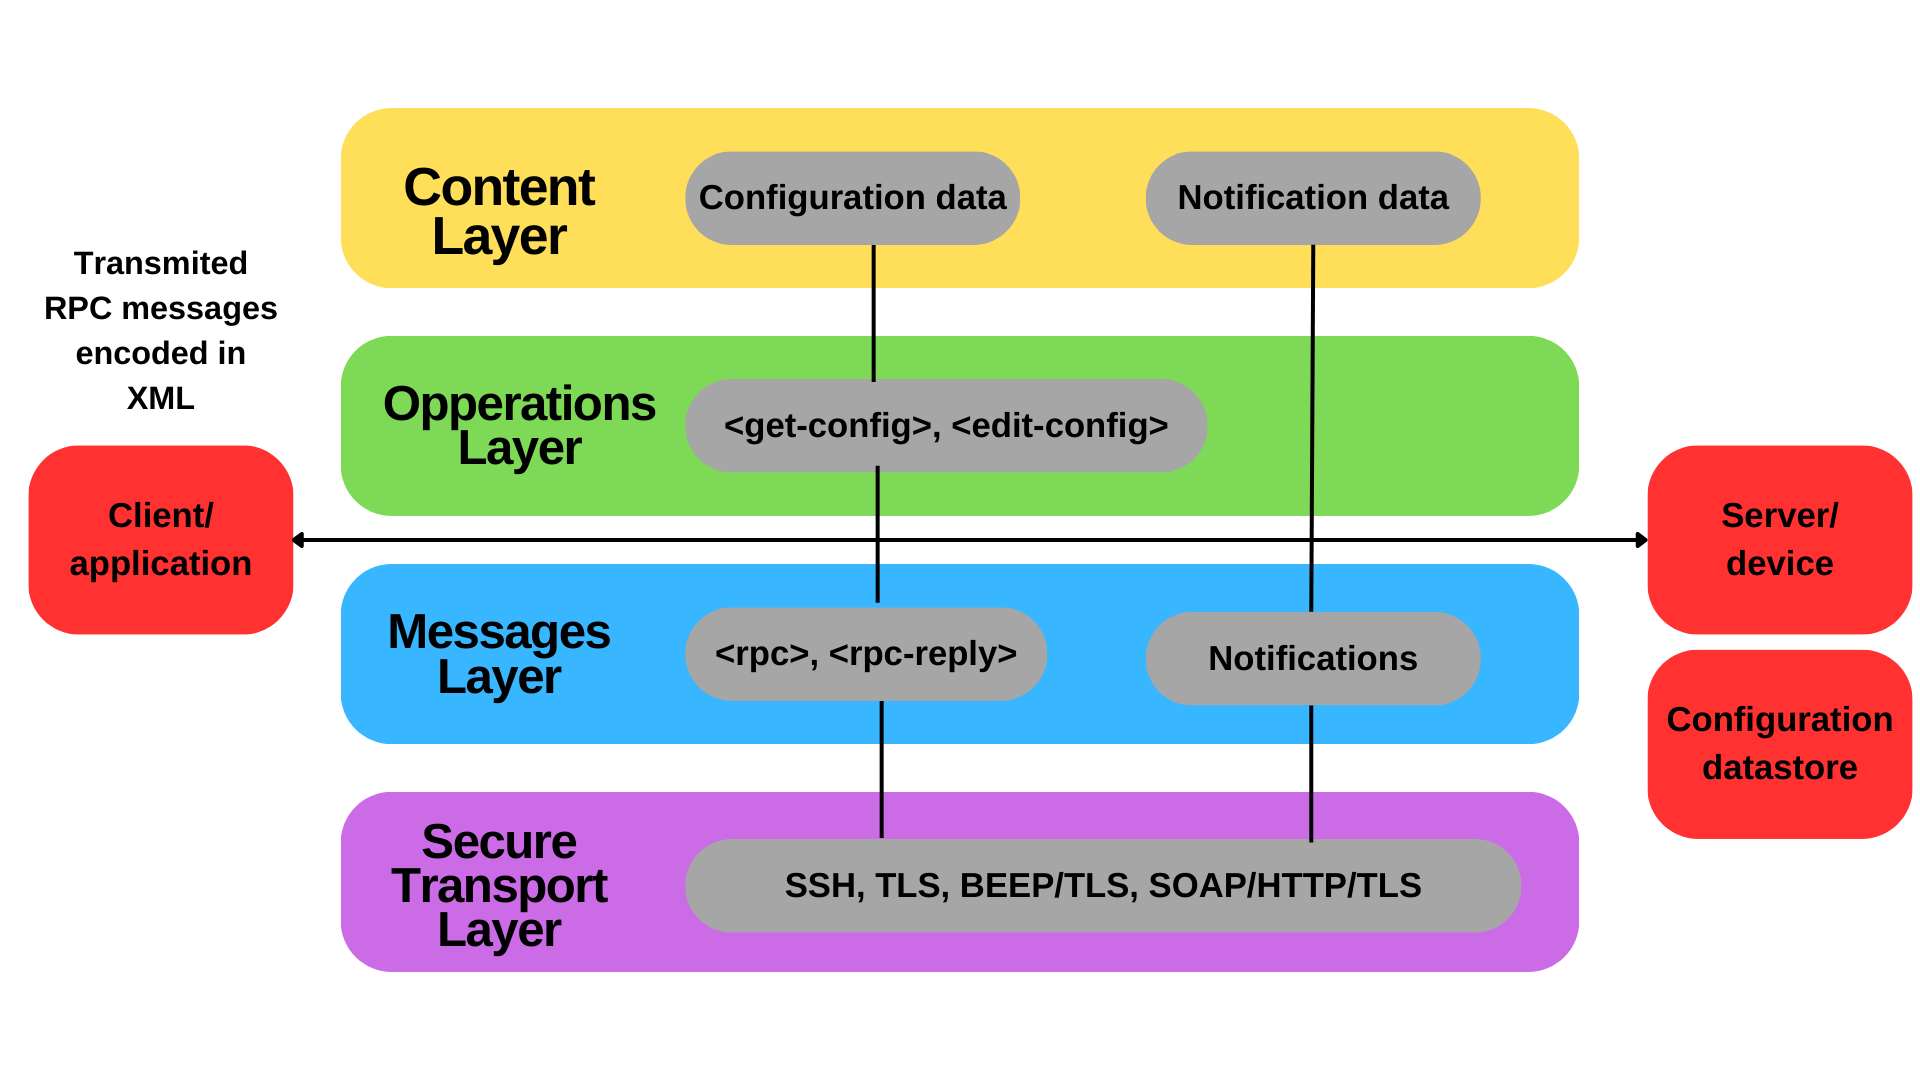
\includegraphics[width=\linewidth]{Images/network_configuration_protocol-f_mobile.png}
    \caption{Diagram illustrating how NETCONF works.}
    \label{fig:example}
\end{figure}

The NETCONF protocol facilitates secure RPC communications between the client and server, providing a standards-based approach to network device management \cite{techtarget}. Figure~\ref{fig:example} provides an overall picture of the NETCONF operation, which can be conceptualized as having four layers as follows:

\begin{itemize}
    \item Secure Transport Layer. The first layer provides the core communication path between the client and server. NETCONF is not bound to any transport protocol, but it can be executed over any transport protocol, including Transport Layer Security and Secure Shell. However, the protocol must provide the necessary functionality. The transport layer makes it possible for the client and server to communicate through a series of RPC messages.
    
    \item Messages Layer. The second layer provides a transport-independent framing mechanism for encoding RPCs and notifications. NETCONF uses an RPC-based communication model to provide the framing necessary to support requests and responses between the client and server. In documenting the Messages Layer, RFC 6241 \cite{rfc6241} focuses primarily on RPC communications, rather than notifications, which are instead documented in RFC 5277 \cite{rfc5277}.
    
    \item Operations Layer. The third layer defines a small set of low-level base operations for retrieving information and managing configurations. The set includes operations such as \texttt{<get-config>} or \texttt{<edit-config>}. The operations are invoked as RPC methods with XML-encoded parameters, passed in as child elements of the RPC elements.
    
    \item Content Layer. The top layer is concerned with configuration and notification data; however, this layer lies outside the scope of RFC 6241. Instead it relies on the device's own data model. NETCONF carries the model's configuration information within the \texttt{<config>} element but treats it as opaque data. The YANG data modeling language, RFC 6020 \cite{6020}, was developed for specifying NETCONF data models and protocol operations.
\end{itemize}

When a client communicates with a server, it sends one or more request messages to that server, which responds with its own reply messages. The two most common XML elements used for RPC communications are \texttt{<rpc>} and \texttt{<rpc-reply>}. The \texttt{<rpc>} element encloses a request sent from the client to the server. The request information within the element includes the RPC's name and its parameters. Then, the \texttt{<rpc-reply>} element is used to respond to the previous messages, and it is sent by the server. All response data is encoded within the \texttt{<rpc-reply>} element.

Within the communication flow of a NETCONF session there are 3 main parts. These are:
\begin{itemize}
    \item Session Establishment: Each side sends a \texttt{<hello>} element, along with another one (\texttt{<capabilities>}) announcing what operations (capabilities) it supports.
    
    \item Operation Request: The client then sends its request (operation) to the server via an \texttt{<rpc>} message. The response is then sent back to the client within an \texttt{<rpc-reply>}.
    
    \item Session Close: The session is then closed by the client via \texttt{<close-session>}.
\end{itemize}

\section{Yet Another Next Generation - YANG}

\gls{YANG} is a data modeling language, providing a standardized way to model the operational and configuration data of a network device. YANG, being a language, is protocol independent, and then can be embedded into any encoding format, e.g. XML or JSON \cite{NETCONFYANG}.


The data models defined in YANG to be used by NETCONF are classified as either Open or Native, with different groups working across each one:

\begin{itemize}
    \item Open Models: These models are designed to be independent of the underlying platform, and so they are vendor agnostic. In turn, different vendors implement the normalization tasks within their devices to process open data models. Open YANG Models are developed by Vendors and Standardization bodies, such as IETF, ITU, OpenConfig etc.
    
    \item Native Models: Native Models are vendor specific. They relate and are designed to integrate to features or configuration only relevant to specific vendors or devices.
\end{itemize}

A YANG model is made up from various components, as depicted in Figure~\ref{fig:yangModels}:

\begin{figure}[h]
    \centering
    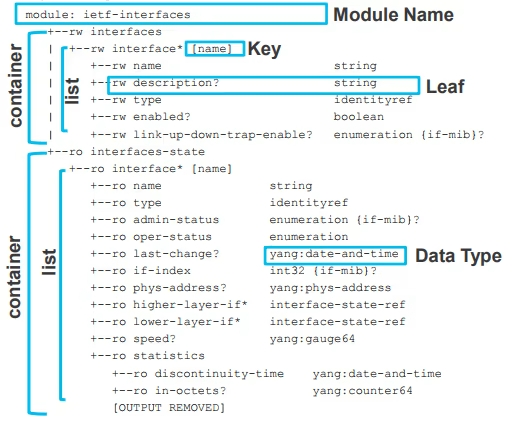
\includegraphics[width=0.7\linewidth]{Images/yang.jpg}
    \caption{Example of a YANG data model structure.}
    \label{fig:yangModels}
\end{figure}


\begin{itemize}
    \item Container: A collection of information logically grouped. For instance there can be a containers defined for configuration, and for state.
    \item List: Within a container you can have a list or even multiple lists. An example would be a list of interfaces.
    \item Key: Each item within the list is referenced via a key.
    \item Leaf: Each element of a list has leafs, which contain the actual information.
    \item Data Type: For each leaf, the data type of the information is indicated.
\end{itemize}

\section{Extensible Markup Language - XML}
Extensible Markup Language (XML) lets us define and store data in a shareable manner. XML supports information exchange between computer systems such as websites, databases, and third-party applications. Predefined rules make it easy to transmit data as XML files over any network because the recipient can use those rules to read the data accurately and efficiently.

In the context of NETCONF, XML is used as the format for exchanging configuration information between the client and the server). NETCONF defines a set of standardized XML-based messages that are used to manage the configuration and operational state of network devices.

When a client sends a request to a network device using NETCONF, it typically includes an XML document that specifies the desired configuration changes or queries. The network device processes the XML request, performs the necessary operations, and sends a response back to the client in XML format.

The use of XML in NETCONF provides several benefits. First, XML is a widely adopted standard for data representation, making it compatible with a variety of systems and tools. Second, XML allows for structured and hierarchical representation of complex network configurations. Finally, the human-readable nature of XML makes it easier for administrators and developers to understand and work with the configuration data.


\section{Remote Procedure Call - RPC}
Remote Procedure Call is a communication protocol that one program can use to request a service from a program located in another computer on a network without having to understand the underlying characteristics. RPC is used to call other processes on the remote systems like a local system. A procedure call is also sometimes known as a function call or a subroutine call.

\subsection*{RPC Model}

The NETCONF protocol uses an RPC-based communication model. NETCONF peers use \texttt{<rpc>} and \texttt{<rpc-reply>} XML elements to provide transport-protocol-independent framing of NETCONF requests and responses.

\subsection*{\texttt{<rpc>} Element}
The \textless{rpc}\textgreater{} element is used to enclose a NETCONF request sent from theclient to the server.

The \texttt{<rpc>} element has a mandatory attribute ``message-id'' which is a string chosen by the sender of the RPC that will commonly encode a monotonically increasing integer. The receiver of the RPC does not decode or interpret this string but simply saves it to be used as a ``message-id'' attribute in any resulting \texttt{<rpc-reply>} message. 

\begin{lstlisting}[style=xmlStyle, caption={\texttt{<rpc>} Model.}, backgroundcolor=\color{codebackground}]
                <rpc message-id="101"
                        xmlns="urn:ietf:params:xml:ns:netconf:base:1.0">
                    <some-method>
                        <!-- method parameters here... -->
                    </some-method>
                </rpc>             
\end{lstlisting}

The name and parameters of an RPC are encoded as the contents of the \texttt{<rpc>} element. The name of the RPC is an element directly inside the \texttt{<rpc>} element, and any parameters are encoded inside this element.

The following example invokes the NETCONF \texttt{<get>} method with no parameters:

\begin{lstlisting}[style=xmlStyle, caption={\texttt{<rpc>} \texttt{<get>} Model.}, backgroundcolor=\color{codebackground}]
                <rpc message-id="101"
                        xmlns="urn:ietf:params:xml:ns:netconf:base:1.0">
                    <get/>
                </rpc>           
\end{lstlisting}




\subsection*{\texttt{<rpc-reply>} Element}


The \texttt{<rpc-reply>} message is sent in response to an \texttt{<rpc>} message.

The \texttt{<rpc-reply>} element has a mandatory attribute ``message-id'', which is equal to the ``message-id'' attribute of the \texttt{<rpc>} for which this is a response.

A NETCONF server MUST also return any additional attributes included in the \texttt{rpc} element unmodified in the \texttt{<rpc-reply>} element.

The response data is encoded as one or more child elements to the \texttt{rpc-reply} element.

For example, the following \texttt{<rpc>} element invokes the NETCONF \texttt{<get>} method and includes an additional attribute called ``user-id''.  Note that the ``user-id'' attribute is not in the NETCONF namespace.  The returned \texttt{<rpc-reply>} element returns the ``user-id'' attribute, as well as the requested content.

\begin{lstlisting}[style=xmlStyle, caption={\texttt{<rpc-reply>} \texttt{<get>} Model.}, backgroundcolor=\color{codebackground}]
                <rpc message-id="101"
                        xmlns="urn:ietf:params:xml:ns:netconf:base:1.0"
                        xmlns:ex="http://example.net/content/1.0"
                        ex:user-id="fred">
                    <get/>
                </rpc>

                <rpc-reply message-id="101"
                    xmlns="urn:ietf:params:xml:ns:netconf:base:1.0"
                    xmlns:ex="http://example.net/content/1.0"
                    ex:user-id="fred">
                    <data>
                        <!-- contents here... -->
                    </data>
                </rpc-reply>         
\end{lstlisting}



